\documentclass{article}

\usepackage[utf8]{inputenc}
\usepackage[ngerman]{babel}

\usepackage{amssymb}
\usepackage{amsmath}

\usepackage{latexsym}
\usepackage{graphicx}

\title{FGI2 Übungen Blatt 1}

\author{Oliver Sengpiel, 6322763 \\ Daniel Speck, 6321317 \\ Daniel
Krempels, 6424833}

\begin{document}

\maketitle

\section*{2.3}
\subsection*{2.3.1}
Die Sprache $L(A_{2.3})$ ist genau die Sprache $L = \{ a\} \{ba^*c\}^* \cup
\{ b\} \{cab\}^* \{c\} \{e , a\}$. \\
Die Sprache $L^\omega(A_{2.3})$ ist genau die Sprache $L^\omega = \{a \} 
\{ba^*c\}^\omega \cup \{ b \}\{cab\}^\omega $. \\
Die Sprache $(L(A_{2.3}))^\omega$ ist genau die Sprache, die Wörter der Form
$((a (ba^*c)^*) + (b (cab)^* c (e + a)))^\omega$ enthält.

\subsection*{2.3.2}
Sowohl $L^\omega (A_{2.3})$, als auch $(L(A_{2.3}))^\omega$ sind
$\omega$-reguläre Mengen. Aber $L^\omega (A_{2.3})$ ist genau die Sprache, die
der Automat $A_{2.3})$ akzeptieren würde, wenn man ihn als Büchi-Automat
ansieht, also die Menge der $\omega$-Worte, die unendlich oft mindestens einen
Endzustand durchlaufen.

$(L(A_{2.3}))^\omega$ bezeichnet hingegen den $\omega$-Abschluss der regulären
Menge $L(A_{2.3}) \setminus \{\varepsilon\}$.

Beispielwörter:\\
$u = abaacbaacbaacbaac \dots \qquad , u \in L^\omega (A_{2.3})$\\
$v = bceabcbceabcbcebc \dots \qquad ,v \in (L(A_{2.3}))^\omega$

\subsection*{2.3.4}
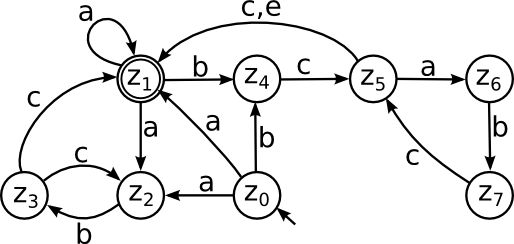
\includegraphics[width=\textwidth]{Automat1.png}

\section*{2.4}
\subsection*{2.4.2}
\begin{enumerate}
\item Man konstruiere einen NFA, der die Menge der Wörter $W$ akzeptiert.
\item Nun konstruiere man einen Büchiautomaten, der $U$ akzeptiert.
\item Als nächstes erhalten alle Endzustände des NFA die
Übergangsrelationen der Startzustände des Büchiautomaten (alle ein- und
ausgehenden Kanten).
\item Der alte Startzustand des Büchiautomaten wird entfernt.
\end{enumerate}

\subsection*{2.4.3}
Zunächst gilt es zu zeigen, dass die Wörter, die unser konstruierter
Automat (nennen wir ihn $A$) akzeptiert in $W\cdot U$ liegen: \\

\underline{$L(A) \subseteq W\cdot U$:}\\
Für unser Wort $w$ gibt es einen Pfad durch den Automaten, der von einem
Startzustand des ehemaligen NFAs zu einem ehemaligen Endzustand des selbigen
führt. Gleichzeitig gibt es für jedes Wort einen Pfad, der von einem
Nachfolgerzustand des ehemaligen alleinstehenden Büchiautomaten zu einer
Schleife durch einen Endzustand führt. Da wir nun Kanten von den ehemaligen
Endzuständen des NFA zu den Nachfolgern der ehemaligen Anfangszustände des
Büchiautomaten konstruiert haben, die das gleiche Eingabesymbol lesen, wie die
alten Kanten des Anfangszustandes, sind die beiden Pfade miteinander verbunden
und ergeben einzelne, lange Pfade, die unendlich oft durch Endzustände führen.

\underline{$W \cdot U \subseteq L(A)$:}\\
Dieses Mal ergibt sich unser Pfad durch das Wort $w$, welches sich aus der
Konkatenation folgender Teile ergibt:
\begin{enumerate}
\item Eine Erfolgsrechnung eines NFA, der $L = W$ akzeptiert
\item Ein Pfad eines Büchiautomaten, der $L = U$ akzeptiert.
\end{enumerate}
Dieser Zusammengesetzte Pfad führt durch den ehemaligen Endzustand unseres
konstruierten NFAs und in einer Schleife durch einen Endzustand unseres
konstruierten Büchiautomaten, die wir miteinander verbunden haben. Dies folgt
aus der Konstruktion, die wir unter $2.4.2$ gemacht haben. 

\subsection*{2.4.4}
Wir wenden unser Verfahren aus $2.4.2$ auf die in der Aufgabe angegebenen
Automaten an.
\begin{enumerate}
\item Konstruiere den Automaten $A_W$:\\
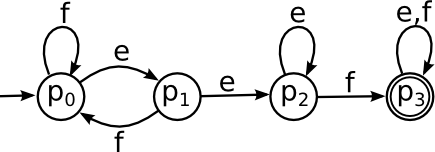
\includegraphics[width=\textwidth]{Aw.png}
\item Konstruiere den Automaten $A_U$:\\
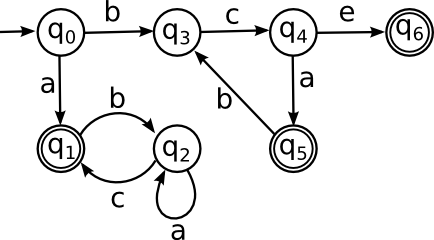
\includegraphics[width=\textwidth]{Au.png}
\item Verbinde alten Endzustand von $A_W$ mit Nachfolgezuständen vom
Anfangszustand von $A_U$ (in dieser Grafik sind die Endzustände von $A_U$ falsch. $q_1$ und
$q_5$ sind auch Endzustände! Im nächsten Bild stimmen die Endzustände wieder):\\
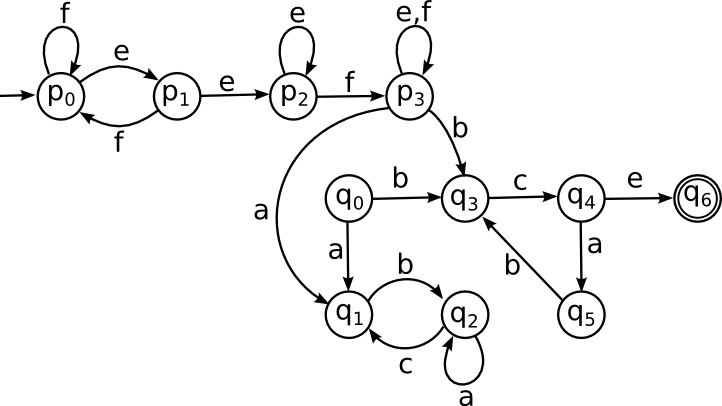
\includegraphics[width=\textwidth]{AwAu1.png}
\item Entfernen des alten Anfangszustandes von $A_U$:\\
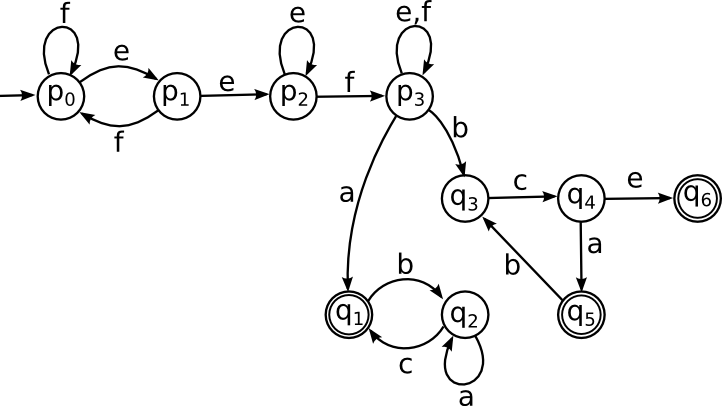
\includegraphics[width=\textwidth]{AwAu2.png}
\end{enumerate}
\end{document}
